% template for poster sections 
% use thie file to create individual sections for a beamer poster 
% then put the pieces together using the poster-template file 

%%%%%%%%%%%%%%%%%%%% 
% top matter 
%%%%%%%%%%%%%%%%%%%% 

%\documentclass[leqno,presentation]{beamer} 
\documentclass[leqno,handout]{beamer}

%\usepackage[orientation=portrait, size=a3, scale=1]{beamerposter} 
\DeclareGraphicsExtensions{.eps, .jpg, .png, .tif} 

\usepackage{calc} 
\usepackage{times} 
\usepackage{type1cm} 
\usepackage[latin1]{inputenc} 
\usepackage{xcolor, colortbl} 
\usepackage{amsmath, amssymb, latexsym} 
\usepackage[english]{babel} 
\usetheme{Darmstadt} 
\usepackage{hyperref} 
\usepackage{gensymb}

% change to location of graphics files, comment out if graphics files 
% are in same directory as tex file 

\graphicspath{{Graphics/}} 

%%%%%%%%%%%%%%%%%%%%%%%%%%%%%%%%%%%%%%%% 
% end top matter, document begins 
%%%%%%%%%%%%%%%%%%%%%%%%%%%%%%%%%%%%%%%% 

\newcommand{\highlight}[1]{ 
\addtolength{\fboxrule}{.2ex} 
\begin{block}{} 
\begin{quote}#1 
\end{quote} 
\end{block} 
} 

\title{Interactive Visualizations \\ with Mathematica} 
	\author{\small{\\[-2.5ex] Faculty Mentor: A.J. Hildebrand \\
    Project Leader: Efstathios Konstantinos Chrontsios Garitsis \\
	IGL Scholars: Xiaojun Jia, Adithya Swaminathan, \\
	Dimitrios Tambakos, Troy Yang, Sarah Zimmerman}}

\institute{\\[-3ex] University of Illinois at Urbana-Champaign 
           \\[2ex] \includegraphics[width = 0.3\textwidth]{uiuc_logo-with-name.png} 
                   \hspace{.30cm} 
                   \includegraphics[width = 0.07\textwidth]{igl-logo-small.png} 
           \\[3ex] Illinois Geometry Lab \\ 
                   Midterm Presentation \\ 
                   March 22, 2021\\ [2ex]} 
\date{} 
\begin{document} 
\frame{\titlepage} 

%%%%%%%%%%%%%%%%%%%% 

\section {Project Goals}
\begin{frame} 

    
\frametitle{Project Goals} 

\begin{itemize}

\item  Create interactive Mathematica-based visualizations of 
fractal-like phenomena arising in number theory and analysis
for use in instruction and outreach activities.

\item Learn more about the mathematics behind these topics.

\item Make the visualizations available to a broader audience through publication at the Wolfram Demonstrations website.

\end{itemize}
\end{frame} 

%%%%%%%%%%%%%%%%%%%% 
%% ALL INFORMATION BEYOND THIS POINT MUST BE EDITED %%
\section {The Julia Set}
\begin{frame} 
	\frametitle{The Julia Set} 
\begin{itemize}
         \item Let P: $\mathbb{C}\rightarrow\mathbb{C}$ be a polynomial and denote $P^{k}$ as the k-th iterate.
            \begin{itemize}
            \item i.e. P $\circ$ P $\circ$ ... $\circ$ P k times.
            \end{itemize}
         \item We define the Julia set to be the boundary of all the points $z \in \mathbb{C}$ for which the set $\{P^{k}(z) : k \in \mathbb{N}\}$ is bounded.
         \item The complement of the Julia set is the Fatou set.
\end{itemize}
\begin{center}
    We are specifically interested in the nature of the Julia Set graph of cubic polynomials as the coefficients vary.
\end{center}


\end{frame}	

\begin{frame} 

    
\frametitle{Julia Set for $z^{2}$ + c when c = 0.25x, $x\in [-3,2] \cap \mathbb{Z}$} 

\begin{itemize}

\item  People have been working a lot on Julia set of $z^{2}$ + c when c changes.

\begin{column}{0.3\textwidth}
      	\begin{center}
        \includegraphics[
        height=0.9\textwidth,
        width=0.9\textwidth]{c=-075.PNG}
        \end{center}
        \begin{center}
        \includegraphics[
        height=0.9\textwidth,
        width=0.9\textwidth,]{c=0.PNG}
        \end{center}
\end{column}
\begin{column}{0.3\textwidth}
      	\begin{center}
        \includegraphics[
        height=0.9\textwidth,
        width=0.9\textwidth,]{c=-05.PNG}
        \end{center}
        \begin{center}
        \includegraphics[
        height=0.9\textwidth,
        width=0.9\textwidth,]{c=025.PNG}
        \end{center}
\end{column}
\begin{column}{0.3\textwidth}
      	\begin{center}
        \includegraphics[
        height=0.9\textwidth,
        width=0.9\textwidth,]{c=-025.PNG}
        \end{center}
        	\begin{center}
        \includegraphics[
        height=0.9\textwidth,
        width=0.9\textwidth,]{c=05.PNG}
        \end{center}
\end{column}

\end{itemize}
\end{frame}

\begin{frame} 

    
\frametitle{Julia Set for $z^{3}+a z^{2} + e^{2 \pi i \theta}z$ \\ when $\theta = \sqrt{2}$, $a\in [-2,2] \cap \mathbb{Z}$} 

\begin{itemize}
\item  When $\lvert a \rvert$ is the same, their graphs are central symmetric.
\\

\begin{column}{0.3\textwidth}
      	\begin{center}
      	\\a = -2
        \includegraphics[
        height=0.75\textwidth,
        width=1\textwidth]{sqrt_2_a=-2.PNG}
        \end{center}
        \begin{center}
        \\a = 2
        \includegraphics[
        height=0.75\textwidth,
        width=1\textwidth,]{sqrt_2_a=2.PNG}
        \end{center}
\end{column}
\begin{column}{0.3\textwidth}
      	\begin{center}
      	\\a = -1
        \includegraphics[
        height=0.75\textwidth,
        width=1\textwidth,]{sqrt_2_a=-1.PNG}
        \end{center}
        \begin{center}
        \\a = 1
        \includegraphics[
        height=0.75\textwidth,
        width=1\textwidth,]{sqrt_2_a=1.PNG}
        \end{center}
\end{column}
\begin{column}{0.3\textwidth}
      	\begin{center}
      	\\a = 0
        \includegraphics[
        height=0.75\textwidth,
        width=1\textwidth,]{sqrt_2_a=0.PNG}
        \end{center}
\end{column}

\end{itemize}

\end{frame}

\begin{frame} 
    
\frametitle{Julia Set for $z^{3}+az^2 + e^{2 \pi i \theta}z$ \\ when $\theta=\pi^\pi$, $a=\{0.59+1.5x \mid x \in \mathbb{Z \}}$}
 
\begin{itemize}
\begin{column}{0.3\textwidth}
\begin{center}
    \\$a=0.59-1.5i$
    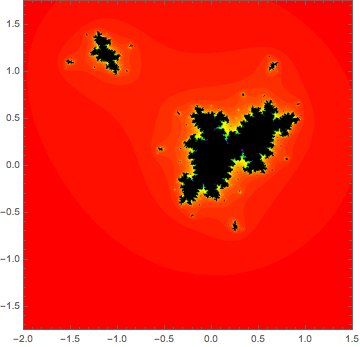
\includegraphics[width=1in,height=1in]{pi2pi1.png}
    \\$a=0.59+4.5i$
    \includegraphics[width=1in,height=1in]{pi2pi5.png} 
\end{center}
\end{column}
\begin{column}{0.3\textwidth}
\begin{center}
    \\$a=0.59$
    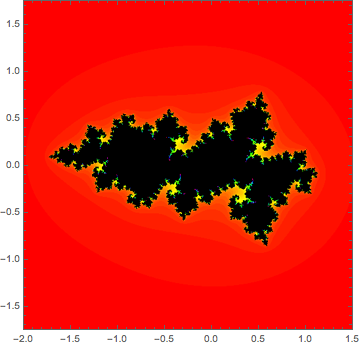
\includegraphics[width=1in,height=1in]{pi2pi2.png} 
    \\$a=0.59+3i$
    \includegraphics[width=1in,height=1in]{pi2pi4.png}
\end{center}
\end{column}
\begin{column}{0.3\textwidth}
    \begin{center}
    $a=0.59+1.5i$
    \includegraphics[
    height=1.2\textwidth,
    width=1.2\textwidth,]{pi2pi3.png}
    \end{center}
\end{column}
\end{itemize}

\end{frame}


\begin{frame} 
    
\frametitle{Julia Set for ${z^3 + a z^2 + e^{2 \pi i \theta} z}$ \\when ${a = 0.2, \theta \in \{e, \phi, \sqrt{2}, \pi\}}$}
\begin{itemize}

\item \small When ${a = 0.2}$ and ${\theta}$ varies, the overall shapes of the graph remain similar, with a rotation.
\\

\begin{column}{0.2\textwidth}
 \begin{center}
    \\${\theta = e}$
    \includegraphics[
        height=1.\textwidth,
        width=1.5\textwidth]{02e.pdf}
    \\${\theta = \sqrt{2}}$
        \includegraphics[
        height=1.\textwidth,
        width=1.5\textwidth]{02sqrt2.pdf}
        \end{center}
    
\end{column}
\begin{column}{0.2\textwidth}
\begin{center}
    \\${\theta = \phi}$
        \includegraphics[
        height=1.\textwidth,
        width=1.5\textwidth]{02gold.pdf}
        \end{center}
        \begin{center}
    \\${\theta = \pi}$
    \includegraphics[
        height=1.\textwidth,
        width=1.5\textwidth]{02pi.pdf}
        \end{center}
    
\end{column}   
\begin{column}{0.2\textwidth}
\end{column}        
\end{itemize}
\end{frame}



\section {Sum-of-Digit Fractals}
\begin{frame} 

    
\frametitle{Sum-of-Digit Fractals} 

\begin{itemize}

\item  \textbf{Sum-of-Digit Function:}
$s_{b}(n)$ denotes the sum of the digits of a number $n$ in base $b$.
\\
\textbf{Example 1:} $s_{10}(15) = 1 + 5 = 6$
\\
\textbf{Example 2:} $s_{2}(15) = s_{2}(1111) = 1 + 1 + 1+ 1 = 4$
%\item \textbf{Exponential Sums with Sum-of-Digit Functions:}
%\[ S_{b, p}(N) = \sum_{n=1}^{N}{e^{2\pi i\, s_{b}(n)/p}}\]

\item \textbf{Sum-of-Digit Fractals:}
Fractals with steps given by 
% the terms of $S_{b, p}(N) = \sum_{n=1}^{N}{e^{2\pi i\, s_{b}(n)/p}}$. Since the terms are complex numbers, we can interpret them as vectors in the $xy$-plane given by:
\[(\cos(2\pi  s_{b}(n)/p), \sin(2\pi s_{b}(n)/p))\]
where $s_b(n)$ is the sum-of-digit function and $p$ is a parameter.

\end{itemize}

\end{frame}

\begin{frame} 

    
\frametitle{Sum-of-Digit Fractals:\\
A Simple Example ($b=2$, $p=7$, $n=5$)} 
{\footnotesize
Using the formula $(\cos(2\pi  s_{b}(n)/p), \sin(2\pi s_{b}(n)/p))$ with $b=2$, $p=7$, and $n=1,2,\dots,5$ we obtain  the first five steps of the curve
corresponding to base $b=2$ and parameter $p=7$. The resulting curve is shown on the right.

\begin{column}{0.48\textwidth}
\begin{itemize}

\item  \textbf{Step 1:}
$(\cos(2 \pi /7), \sin(2 \pi /7))$.
\item \textbf{Step 2:}
 $(\cos(2 \pi /7), \sin(2 \pi /7))$.


\item \textbf{Step 3:}
 $(\cos(4 \pi /7), \sin(4 \pi /7))$.

\item \textbf{Step 4:}
$(\cos(2 \pi /7), \sin(2 \pi /7))$.

\item \textbf{Step 5:}
$(\cos(4 \pi /7), \sin(4 \pi /7))$.

\end{itemize}
\end{column}
}
\begin{column}{0.5\textwidth}

\begin{center}
        \includegraphics[
        width=0.95\textwidth,
        height=0.4\textheight]{arrows.png}
               \end{center}
    \end{column}   
\end{frame} 

\begin{frame}

\frametitle{Sum-of-Digit Fractals ($b \equiv 1 \pmod{p}$)} 

\begin{center}
($p = 3$) \includegraphics[width=1.5in,height=1.25in]{trianglewalk.png}
\hspace{0.2in} \includegraphics[width=1.5in,height=1.25in]{square.png} ($p = 4$)\\
($p = 5$) \includegraphics[width=1.5in,height=1.25in]{pentagon.png} 
\hspace{0.2in} \includegraphics[width=1.5in,height=1.25in]{hexagon.png} ($p = 6$)
\\[0.1in] If $b$ is one greater than a multiple of $p$, we get a regular $p$-gon. \end{center}
    
\end{frame}

\begin{frame}

\frametitle{Sum-of-Digit Fractals ($b = p$)} 

\begin{center}
($p = 3$) \includegraphics[width=1.25in,height=1.0in]{bequalsn3.png}
\hspace{0.2in} \includegraphics[width=1.25in,height=1.0in]{bequalsn4.png}($p=4$)
\\
($p = 5$) \includegraphics[width=1.25in,height=1.0in]{bequalsn5.png}
\hspace{0.2in} \includegraphics[width=1.25in,height=1.0in]{bequalsn6.png}($p=6$)
\\[0.1in] If $b$ is equal to $p$, we get $p$ number of $p$-gons with at least one common vertex. \end{center}
    
\end{frame}

\begin{frame} 

    
% \frametitle{Sum-of-Digit Fractals ($p = 4, N = 2^{13}, b = 2$)} 

% \begin{center}
%         \includegraphics[
%         height=0.7\textheight,
%         width=1\textwidth]{n2carat13b2p4.pdf}
%         \\
%         \end{center}
% \end{frame} 

% \begin{frame} 

    
% \frametitle{Sum-of-Digit Fractals ($N = 10000, b = 12$) } 

% \begin{center}
%         \includegraphics[
%         height=0.45\textheight,
%         width=0.45\textwidth]{halfpiplot.pdf}
%         \hspace{0.2in}
%         \includegraphics[
%         height=0.45\textheight,
%         width=0.45\textwidth]{elevenseven.png}
%         \\[0.1in] Left: $p = \frac{\pi}{2}$. Right: $p = \frac{11}{7}$.
%         \\[0.1in] The similarity is because $\frac{22}{7}$ is a
%         \\ good rational approximation of $\pi$.
%         \end{center}
% \end{frame} 

% \begin{frame} 

    
    
%%%%%%%%   
%\frametitle{Sum-of-Digit Fractals ($p = 2 \pi, N = 1000, b = 3$)} 

% \begin{center}
%         \includegraphics[
%         height=0.7\textheight,
%         width=1\textwidth]{2piplot.pdf}
%         \\
%         \end{center}
% \end{frame} 

% \begin{frame} 

    
% \frametitle{Sum-of-Digit Fractals ($p = 3 \pi, N = 100, b = 6$) } 

% \begin{center}
%         \includegraphics[
%         height=0.7\textheight,
%         width=1\textwidth]{3piwalk.png}
%         \\
%         \end{center}
% \end{frame} 

% \begin{frame} 

%%%%%%%%%%%%%
\frametitle{Sum-of-Digit Fractals ($p = 4 \pi, N = 1000, b = 10$)} 

\begin{center}
        \includegraphics[
        height=0.7\textheight,
        width=1\textwidth]{4piplot.pdf}
        \\
        \end{center}
\end{frame} 






%%%%%%%%%%%%%%%%%%%% 




%%%%%%%%%%%%%%%%%%%%



%%%%%%%%%%%%%%%%%%%%


%%%%%%%%%%%%%%%%%%%%



%%%%%%%%%%%%%%%%%%%%


%%%%%%%%%%%%%%%%%%%




%%%%%%%%%%%%%%%%%%%%

\begin{frame} 

    
\frametitle{Next Steps} 


	\begin{itemize}

	    \item Refine code for these visualizations, adding more functionality
	    \item Make these visualizations interactive
	    \item Add more interesting visualizations to the existing set
	    \item Try to prove/explain some of the observed behavior

    \end{itemize}
	

\end{frame} 

%%%%%%%%%%%%%%%%%%%% 



\end{document} 
